%% abtex2-modelo-trabalho-academico.tex, v-1.9.2 laurocesar
%% Copyright 2012-2014 by abnTeX2 group at http://abntex2.googlecode.com/ 
%%
%% This work may be distributed and/or modified under the
%% conditions of the LaTeX Project Public License, either version 1.3
%% of this license or (at your option) any later version.
%% The latest version of this license is in
%%   http://www.latex-project.org/lppl.txt
%% and version 1.3 or later is part of all distributions of LaTeX
%% version 2005/12/01 or later.
%%
%% This work has the LPPL maintenance status `maintained'.
%% 
%% The Current Maintainer of this work is the abnTeX2 team, led
%% by Lauro César Araujo. Further information are available on 
%% http://abntex2.googlecode.com/
%%
%% This work consists of the files abntex2-modelo-trabalho-academico.tex,
%% abntex2-modelo-include-comandos and abntex2-modelo-references.bib
%%

% ------------------------------------------------------------------------
% ------------------------------------------------------------------------
% abnTeX2: Modelo de Trabalho Academico (tese de doutorado, dissertacao de
% mestrado e trabalhos monograficos em geral) em conformidade com 
% ABNT NBR 14724:2011: Informacao e documentacao - Trabalhos academicos -
% Apresentacao
% ------------------------------------------------------------------------
% ------------------------------------------------------------------------

\documentclass[
	% -- opções da classe memoir --
	12pt,				% tamanho da fonte
	openright,			% capítulos começam em pág ímpar (insere página vazia caso preciso)
	twoside,			% para impressão em verso e anverso. Oposto a oneside
	a4paper,			% tamanho do papel. 
	% -- opções da classe abntex2 --
	%chapter=TITLE,		% títulos de capítulos convertidos em letras maiúsculas
	%section=TITLE,		% títulos de seções convertidos em letras maiúsculas
	%subsection=TITLE,	% títulos de subseções convertidos em letras maiúsculas
	%subsubsection=TITLE,% títulos de subsubseções convertidos em letras maiúsculas
	% -- opções do pacote babel --
	english,			% idioma adicional para hifenização
	french,				% idioma adicional para hifenização
	spanish,			% idioma adicional para hifenização
	brazil				% o último idioma é o principal do documento
	]{abntex2}

% ---
% Pacotes básicos 
% ---
\usepackage{lmodern}			% Usa a fonte Latin Modern			
\usepackage[T1]{fontenc}		% Selecao de codigos de fonte.
\usepackage[utf8]{inputenc}		% Codificacao do documento (conversão automática dos acentos)
\usepackage{lastpage}			% Usado pela Ficha catalográfica
\usepackage{indentfirst}		% Indenta o primeiro parágrafo de cada seção.
\usepackage{color}				% Controle das cores
\usepackage{graphicx}			% Inclusão de gráficos
\usepackage{microtype} 			% para melhorias de justificação
% ---
		
% ---
% Pacotes adicionais, usados apenas no âmbito do Modelo Canônico do abnteX2
% ---
\usepackage{lipsum}				% para geração de dummy text
% ---

% ---
% Pacotes de citações
% ---
\usepackage[brazilian,hyperpageref]{backref}	 % Paginas com as citações na bibl
\usepackage[alf]{abntex2cite}	% Citações padrão ABNT

% --- 
% CONFIGURAÇÕES DE PACOTES
% --- 

% ---
% Configurações do pacote backref
% Usado sem a opção hyperpageref de backref
\renewcommand{\backrefpagesname}{Citado na(s) página(s):~}
% Texto padrão antes do número das páginas
\renewcommand{\backref}{}
% Define os textos da citação
\renewcommand*{\backrefalt}[4]{
	\ifcase #1 %
		Nenhuma citação no texto.%
	\or
		Citado na página #2.%
	\else
		Citado #1 vezes nas páginas #2.%
	\fi}%
% ---

% ---
% Informações de dados para CAPA e FOLHA DE ROSTO
% ---
\titulo{Chuveiro com aquecimento indutivo}
\autor{Igor Macedo Quintanilha\\Roberto de Moura Estevão Filho}
\local{Rio de Janeiro}
\data{2013.2}
\orientador{Casé}
\coorientador{Joarez}
\instituicao{%
  Universidade Federal do Rio de Janeiro - UFRJ
  \par
  Escola Politécnica
  \par
  Departamento e Engenharia Eletrônica e de Computação
  \par
  Projeto Integrado}
\tipotrabalho{Tese (Doutorado)}
% O preambulo deve conter o tipo do trabalho, o objetivo, 
% o nome da instituição e a área de concentração 
\preambulo{Modelo canônico de trabalho monográfico acadêmico em conformidade com
as normas ABNT apresentado à comunidade de usuários \LaTeX.}
% ---


% ---
% Configurações de aparência do PDF final

% alterando o aspecto da cor azul
\definecolor{blue}{RGB}{41,5,195}

% informações do PDF
\makeatletter
\hypersetup{
     	%pagebackref=true,
		pdftitle={\@title}, 
		pdfauthor={\@author},
    	pdfsubject={\imprimirpreambulo},
	    pdfcreator={LaTeX with abnTeX2},
		pdfkeywords={abnt}{latex}{abntex}{abntex2}{trabalho acadêmico}, 
		colorlinks=true,       		% false: boxed links; true: colored links
    	linkcolor=blue,          	% color of internal links
    	citecolor=blue,        		% color of links to bibliography
    	filecolor=magenta,      		% color of file links
		urlcolor=blue,
		bookmarksdepth=4
}
\makeatother
% --- 

% --- 
% Espaçamentos entre linhas e parágrafos 
% --- 

% O tamanho do parágrafo é dado por:
\setlength{\parindent}{1.3cm}

% Controle do espaçamento entre um parágrafo e outro:
\setlength{\parskip}{0.2cm}  % tente também \onelineskip

% ---
% compila o indice
% ---
\makeindex
% ---

% ----
% Início do documento
% ----
\begin{document}

% Retira espaço extra obsoleto entre as frases.
\frenchspacing 

% ----------------------------------------------------------
% ELEMENTOS PRÉ-TEXTUAIS
% ----------------------------------------------------------
% \pretextual

% ---
% Capa
% ---
\imprimircapa
% ---

% ---
% Folha de rosto
% (o * indica que haverá a ficha bibliográfica)
% ---
\imprimirfolhaderosto
% ---


% ---
% Inserir errata
% ---
\begin{errata}
Elemento opcional da \citeonline[4.2.1.2]{NBR14724:2011}. Exemplo:

\vspace{\onelineskip}

FERRIGNO, C. R. A. \textbf{Tratamento de neoplasias ósseas apendiculares com
reimplantação de enxerto ósseo autólogo autoclavado associado ao plasma
rico em plaquetas}: estudo crítico na cirurgia de preservação de membro em
cães. 2011. 128 f. Tese (Livre-Docência) - Faculdade de Medicina Veterinária e
Zootecnia, Universidade de São Paulo, São Paulo, 2011.

\begin{table}[htb]
\center
\footnotesize
\begin{tabular}{|p{1.4cm}|p{1cm}|p{3cm}|p{3cm}|}
  \hline
   \textbf{Folha} & \textbf{Linha}  & \textbf{Onde se lê}  & \textbf{Leia-se}  \\
    \hline
    1 & 10 & auto-conclavo & autoconclavo\\
   \hline
\end{tabular}
\end{table}

\end{errata}
% ---

% ---
% Inserir folha de aprovação
% ---

% Isto é um exemplo de Folha de aprovação, elemento obrigatório da NBR
% 14724/2011 (seção 4.2.1.3). Você pode utilizar este modelo até a aprovação
% do trabalho. Após isso, substitua todo o conteúdo deste arquivo por uma
% imagem da página assinada pela banca com o comando abaixo:
%
% \includepdf{folhadeaprovacao_final.pdf}
%
%\begin{folhadeaprovacao}

%  \begin{center}
%    {\ABNTEXchapterfont\large\imprimirautor}

%    \vspace*{\fill}\vspace*{\fill}
%    \begin{center}
%      \ABNTEXchapterfont\bfseries\Large\imprimirtitulo
%    \end{center}
%    \vspace*{\fill}
    
%   \hspace{.45\textwidth}
%    \begin{minipage}{.5\textwidth}
%        \imprimirpreambulo
%    \end{minipage}%
%    \vspace*{\fill}
%   \end{center}
        
  % Trabalho aprovado. \imprimirlocal, 24 de novembro de 2012:

 %  \assinatura{\textbf{\imprimirorientador} \\ Professor} 
 %  \assinatura{\textbf{Professor} \\ Convidado 1}
%   \assinatura{\textbf{Professor} \\ Convidado 2}
   %\assinatura{\textbf{Professor} \\ Convidado 3}
   %\assinatura{\textbf{Professor} \\ Convidado 4}
      
%   \begin{center}
%    \vspace*{0.5cm}
%    {\large\imprimirlocal}
%    \par
%    {\large\imprimirdata}
%    \vspace*{1cm}
%  \end{center}
  
%\end{folhadeaprovacao}
% ---

% ---
% Dedicatória
% ---
\begin{dedicatoria}
   \vspace*{\fill}
   \centering
   \noindent
   \textit{ Este trabalho é dedicado às crianças adultas que,\\
   quando pequenas, sonharam em se tornar cientistas.} \vspace*{\fill}
\end{dedicatoria}
% ---

% ---
% Agradecimentos
% ---
\begin{agradecimentos}

\end{agradecimentos}
% ---

% ---
% inserir lista de ilustrações
% ---
\pdfbookmark[0]{\listfigurename}{lof}
\listoffigures*
\cleardoublepage
% ---

% ---
% inserir lista de tabelas
% ---
\pdfbookmark[0]{\listtablename}{lot}
\listoftables*
\cleardoublepage
% ---

% ---
% inserir lista de abreviaturas e siglas
% ---
\begin{siglas}
  \item[ABNT] Associação Brasileira de Normas Técnicas
  \item[abnTeX] ABsurdas Normas para TeX
\end{siglas}
% ---

% ---
% inserir lista de símbolos
% ---
\begin{simbolos}
  \item[$ \Gamma $] Letra grega Gama
  \item[$ \Lambda $] Lambda
  \item[$ \zeta $] Letra grega minúscula zeta
  \item[$ \in $] Pertence
\end{simbolos}
% ---

% ---
% inserir o sumario
% ---
\pdfbookmark[0]{\contentsname}{toc}
\tableofcontents*
\cleardoublepage
% ---



% ----------------------------------------------------------
% ELEMENTOS TEXTUAIS
% ----------------------------------------------------------
\textual

% ----------------------------------------------------------
% 
% ----------------------------------------------------------
\chapter*[Introdução]{Introdução}
\addcontentsline{toc}{chapter}{Introdução}
% ----------------------------------------------------------

\chapter*[Introdução]{Introdução}
\addcontentsline{toc}{chapter}{Introdução}
O chuveiro elétrico é adotado por 73.1\% dos brasileiros, segundo dados da PROCEL\footnote{Programa Nacional de Conservação de Energia Elétrica}\cite{procel2007avaliaccao}, principalmente pelo seu baixo investimento inicial. O alto custo em obras para instalação de gás, solar e outros, faz com que o chuveiro elétrico seja o preferido da população brasileira. No entanto, o chuveiro elétrico convencional carece de uma boa manutenibilidade, devido à necessidade constante de troca da resistência; possui baixa relação temperatura-vazão quando comparado a soluções como aquecimento a gás; além do risco de choques. Por isso, tivemos a ideia de aplicar a tecnologia de aquecimento por indução na criação de um chuveiro. O chuveiro de aquecimento por indução tem como intuito manter a grande vantagem do chuveiro elétrico, mas prover um banho com a qualidade de técnicas que requerem uma instalação mais custosa.

Este trabalho contém uma breve introdução sobre os princípios do aquecimento por indução, diferentes topologias de osciladores usados para gerar a corrente alternada usada no aquecedor, os componentes usados na construção de um protótipo, além de sua montagem, e, por fim, serão discutidos os resultados do projeto.

% ---
% 
% ---
\chapter{Capítulo 1}
\section{Oscilador LC MOS cruzado acoplado}
Neste tipo de oscilador, os transistores est�o em classe A, fornecendo energia ao tanque LC, que consome devido a sua n�o idealidade. Neste caso, a energia que o transistor injeta no tanque, deve ser maior ou igual que a resist�ncia de perda total do circuito. O fator de qualidade deste circuito �:
\begin{equation}
Q = \frac{2\pi*f*L}{R_p}
\end{equation}
E o g_m �:
\begin{equation}
g_m = \frac{i_D}{V_{GS} - V_t}
\end{equation}
Para que ocorra uma oscila��o:
\begin{equation}
\frac{1}{g_m} \geq \frac{2\pi*f*L}{Q}
\end{equation}
� importante notar que, mesmo que o circuito seja inst�vel e os transistores entrem em corte e satura��o, a tesn�o na sa�da continuar� pr�xima de uma senoide perfeita quanto maior for o fator de qualidade do tanque.
Uma das grandes desvantagens desse circuito deve-se ao fato de que s�o poucos os MOSFETs que sustentam uma tens�o de gate maior que 20V, limitando assim a pot�ncia do circuito.


\section{Oscilador Royer}
Em 1954, George Royer patenteou o oscilador Royer, um circuito auto ressonante, simples e com pouco uso de componentes. Como a maioria dos osciladores, ele utiliza um tanque LC para a oscila��o. A grande vantagem deste circuito deve-se ao fato do terceiro enrolamento estar conectado � base dos transistores. Isto garante que um transistor estar� cortado enquanto o outro estiver ativo, diminuindo bastante o consumo energ�tico do circuito.


\section{Oscilador Mazzilli}
O oscilador Mazzilli � uma deriva��o do oscilador Royer com o LC MOS. A grande diferen�a neste circuito est� no circuito presente no gate, para assegurar o baixo consumo energ�tico e o chaveamento em ZVS sem ter que utilizar um terceiro enrolamento no indutor. Mazzilli usa uma combina��o, retirando energia de Vin (como no Royer) e no entanto ligando os gates por um diodo ao dreno oposto. Com isso, suprimos o problema de tens�o que existia no LC MOS e continuamos a utilizasr MOSFET ao inv�s de BJT, podendo assim, garantir alta frequ�ncia na oscila��o.

\subsection{Modos de Opera��o}
Esse convers�o possui quatro modos de opera��o. O primeiro dele consiste no dreno das duas chaves aterrados. Como eles est�o ligados cruzado, isto garante que a chave 1 est� cortada e a 2 ativa. Durante esta opera��o o capacitor � completamente descarregado. Depois disso a chave 1 � cortada e � a vez da chave 2 est� ativa. Assim h� a gera��o de uma corrente que ir� percorrer o tanque LC e ir� descarregar na chave ativa. Quando a voltagem no dreno 1 retorna para zero, ocorre o chaveamento das duas chaves. Assim como no modo de opera��o 1 o capacitor est� completamente descarregado, e o indutor carrega totalmente a corrente em posi��o oposta. E finalmente, o modo 4 que ocorre exatamente o mesmo evento que o modo 2, no entanto, na chave 1.

\subsection{Limita��es do circuito}

\subsubsection{Depend�ncia da carga}
Durante a transfer�ncia de pot�ncia a carga � refletida para o prim�rio, e aparece em paralelo com o tanque LC, e com isso a frequ�encia de oscila��o � dependente da carga em uso, gerando uma perda maior.
\subsubsection{Resposta do Gate}
Quando a frequ�ncia de oscila��o � baixa, este fator n�o � crucial. No entanto, com o aumento de frequ�ncia, j� que o gate � um capacitor, a constante RC deve ser levada em conta.

\subsubsection{Alta voltagem no Gate}
Outro problema � a alta voltagem presente no gate. Este problema � facilmente mitigado adicionando um zener com uma tens�o ligeiramente abaixo da tens�o de breakdown do gate, embora cause uma perda maior na resist�ncia do gate.

\subsection{Resist�ncia do transistor}
Quando o transistor est� descarregando o capacitor, toda a corrente gerada no circuito passa atrav�s dele, havendo a necessidade de optar por um MOSFET que possua a menor resist�ncia poss�vel quando ele estiver ativo, afim de manter a menor perda poss�vel no transistor, e garantir que ele n�o esquente demais.
% ---

% ---
% 
% ---
\chapter{Capítulo 2}
\section{Aquecimento por indu��o}
\subsection{Efeito skin}
\subsection{Histerese}
\subsection{Efici�ncia de aquecimento} %qual a frequencia de oscila��o correta
% ---

% ---
\chapter{Montagem Experimental}
A primeira abordagem para realizar a montagem experimental foi construir uma placa de circuito impresso com o circuito do Mazzilli. Porém, o circuito planejado drenaria uma corente de 30A e oscilaria numa frequência em torno de 400kHz. Utilizando [] para calcular qual deveria ser o tamanho da trilha, chegamos a valores que não seriam práticos. Portanto a ideia era fazer a montagem em outro material e fazer as ligações por cabos que se usam em instalação elétrica, garantindo assim o funcionamento adequado. Para isto, foi feita a montagem experimental em cima de uma placa de madeira, que é um péssimo condutor, funcionando como um ótimo isolante. 
\section{Transistores}
Para podermos atender os requisitos citados em [] foi necessário a escolha de um IRFP250N, onde podemos conferir suas especificações [] na tabela X.


\begin{table}[htb]
\IBGEtab{%
  \caption{Características do IRFP250N}%
  \label{tabela-car-irfp}
}{%
  \begin{tabular}{cccccc}
  \toprule
  & Parâmetro & Valor & Unidade \\
  \midrule
  $I_{DMáx}$ & Corrente contínua de Dreno & 30 & A \\
  $P_{DMáx}$ & Dissipação de potência & 214 & W \\
  $V_{GS}$ & Tensão de gate para source & \pm 20 & V \\
  \bottomrule
\end{tabular}%
}{%
  \fonte{International Rectifier}%
  \nota{Os valores máximos são para uma temperatura de $25^oC$.}%
  %\nota[Anotações]{* Existem os capacitores eletrolíticos %bipolares porém não possuem capacitâncias tão altas.}%
  }
\end{table}


\section{Capacitores}
Outro problema prático é que o capacitor deve ser apolar, pois o sinal excursionado nele ora é positivo, ora é negativo. Além disto, a corrente AC que passa está na ordem de dezenas de amperes, havendo a necessidade de realizar associações em paralelo para dividir a corrente entre os componentes até um valor aceitável. A \ref{tabela-cap-comp} mostra os materiais que são comumente fabricados o capacitor. Podemos observar que o melhor material para agir em conjunto com um circuito que irá oscilar em alta frequência, com uma alta tensão e maior fator de qualidade possível, é o polipropileno. No projeto, foi utilizado 3 capacitores, modelo XXXX [].


\begin{table}[htb]
\IBGEtab{%
  \caption{Comparativo entre os tipos de capacitores.}%
  \label{tabela-cap-comp}
}{%
  \begin{tabular}{cccccc}
  \toprule
  Tipo & Polaridade & Potência & Escala & ESR & Frequência de Operação \\
  \midrule
  Cerâmica & Não & Baixa & $\mu F$ & Baixo & Alta \\
  Poliestireno & Não & Alta & $pF$ & Baixo & Muito Alta \\
  Poliester & Não	& Alta & $\mu F$ & Baixo & Muito Alta \\
  Polipropilêno & Não & Alta & $\mu F$ & Muito baixo & Muito Alta \\
  Eletrolítico & Não* & Alta & $F$ & Alta & Baixa \\
  \bottomrule
\end{tabular}%
}{%
  \fonte{Wikipédia}%
  \nota{\hyphenation{Equivalent Series Resistence }: uma medida de não idealidade do componente que mede o valor da resistência em série com o mesmo para uma determinada frequência.}%
  \nota[Anotações]{* Existem os capacitores eletrolíticos bipolares porém não possuem capacitâncias tão altas.}%
  }
\end{table}



\section{Bobina de Trabalho}

\section{Choke}
Utilizando a fórmula aproximada de Wheeler [], adaptado em [], para ficar em metros e Henrys, temos que a fórmula explicita para o cálculo da indutância é:
\begin{equation}
L = \mu_0 \frac{\pi r^2 n^2}{h + 0.9r}
\end{equation}
Onde $ L$ é a indutância desejada, $\mu_0$ é a permeabilidade no ar, $r$ o raio da seção de reta do indutor, $n$ o número de espiras e $h$ a altura da bobina. Variando os parâmetros $r$, $h$ e $L$, considerando $h = 1.5r$, temos a Figura \ref{fig_comp-indutor}.

\begin{figure}[htb]
\caption{\label{fig_comp-indutor}Número de espiras variando os parâmetros para um indutor de núcleo de ar}
\begin{center}
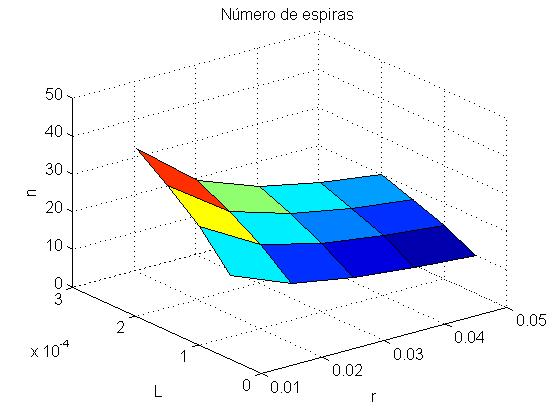
\includegraphics[scale=0.5]{images/comp-indutor.jpg}
\end{center}
\legend{O raio está variando de 1 a 5cm, enquanto a indutância varia de 50 a 200 $\mu H$ }
\end{figure}

Podemos observar que para uma bobina pequena temos que aumentar exponencialmente o número de espiras, além de tomar todo o cuidado para termos um espaçamento e seção de reta uniforme em cada espira. Para sanar o problema, recorremos ao uso de choques com núcleo de ferrite, comumente encontrado em fontes chaveadas. O ferrite possuí como característica alta permeabilidade magnética, baixa condutividade elétrica (prevenindo correntes parasitas) e baixa perda em alta frequência, garantido assim um menor $n$ e consequentemente um menor tamanho de choque. Encontramos a bobina em uma fonte ATX, muito utilizada em computadores (ver Figura \ref{fig_fonte-atx}).

\begin{figure}[htb]
\caption{\label{fig_fonte-atx}Demonstração do choke na fonte ATX}
\begin{center}
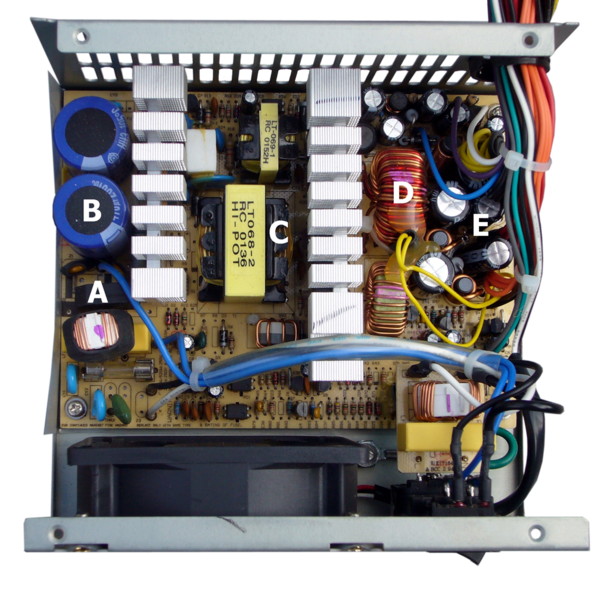
\includegraphics[scale=0.5]{images/fonte-atx.png}
\end{center}
\legend{Observe o choke, marcado com a letra 'D', de uma fonte ATX com núcleo de ferrite enrolado com várias espiras. Fonte: Wikipedia.}
\end{figure}


\section{Diodo de recuperação rápida}
O diodo que realiza o chaveamento do transistor no momento certo, ajudando a descarregar a base, deve poder responder na mesma velocidade de chaveamento necessária no circuito, com isso utilizamos o diodo BYV26A, que tem como principais aplicações, inversores em alta frequência e fontes chaveadas.
\section{Fonte}
Um dos fatores cruciais do projeto é a fonte de alimentação. Ela deve ser capaz de fornecer uma energia de NNNW, uma corrente de XXXXA e ideal seria uma tensão regulada. No entanto, como o projeto em si é uma prova de conceito, não foi possível conseguir uma fonte de tensão regulável. Por fim, utilizamos uma bateria de chumbo, modelo XXXX, de XXXXXXAh. (ver foto)
\section{Montagem}
Utilizamos solda de estanho e fios de $XXmmm^2$ e $XXmm^2$ para a parte de baixa e alta tensão, respectivamente. A montagem final pode ser conferida na figura XX.
% ---

% ----------------------------------------------------------
% Finaliza a parte no bookmark do PDF
% para que se inicie o bookmark na raiz
% e adiciona espaço de parte no Sumário
% ----------------------------------------------------------
\phantompart

% ---
% Conclusão (outro exemplo de capítulo sem numeração e presente no sumário)
% ---
\chapter*[Conclusão]{Conclusão}
\addcontentsline{toc}{chapter}{Conclusão}
% ---

\chapter{Resultados}
Após realizarmos testes no circuito montado, verificamos que o circuito de fato aquecia objetos metálicos. No entanto, devido à operação em potência relativamente baixa, apenas materiais ferromagnéticos tiveram aquecimento expressivo, o que nos leva a concluir que o efeito de histerese é o principal fator para o aquecimento. As correntes de Foucault não dissipam calor significativo mesmo após exposição prolongada ao campo eletromagnético. Foram feitos testes com ferro, alumínio e cobre e apenas materiais de ferro foram aquecidos.

Devido a limitações de tensão da fonte, não foi possível a operação em potências maiores que $216$W, já que com tensão de apenas $12$V, a corrente ficaria demasiadamente elevada. Testes com correntes mais altas levaram a danos nos transistores, que tiveram que ser substituídos.

Apesar do limite de potência, pudemos validar o experimento como prova de conceito, e imaginamos que com potências da ordem de grandeza de um chuveiro elétrico convencional, um chuveiro por aquecimento indutivo seja realizável.

% ----------------------------------------------------------
% ELEMENTOS PÓS-TEXTUAIS
% ----------------------------------------------------------
\postextual
% ----------------------------------------------------------

% ----------------------------------------------------------
% Referências bibliográficas
% ----------------------------------------------------------
\bibliography{referencias}

% ----------------------------------------------------------
% Glossário
% ----------------------------------------------------------
%
% Consulte o manual da classe abntex2 para orientações sobre o glossário.
%
%\glossary

% ----------------------------------------------------------
% Apêndices
% ----------------------------------------------------------

% ---
% Inicia os apêndices
% ---
\begin{apendicesenv}

% Imprime uma página indicando o início dos apêndices
\partapendices

% ----------------------------------------------------------
\chapter{Quisque libero justo}
% ----------------------------------------------------------

\lipsum[50]

% ----------------------------------------------------------
\chapter{Nullam elementum urna vel imperdiet sodales elit ipsum pharetra ligula
ac pretium ante justo a nulla curabitur tristique arcu eu metus}
% ----------------------------------------------------------
\lipsum[55-57]

\end{apendicesenv}
% ---


% ----------------------------------------------------------
% Anexos
% ----------------------------------------------------------

% ---
% Inicia os anexos
% ---
\begin{anexosenv}

% Imprime uma página indicando o início dos anexos
\partanexos

% ---
\chapter{Morbi ultrices rutrum lorem.}
% ---
\lipsum[30]

% ---
\chapter{Cras non urna sed feugiat cum sociis natoque penatibus et magnis dis
parturient montes nascetur ridiculus mus}
% ---

\lipsum[31]

% ---
\chapter{Fusce facilisis lacinia dui}
% ---

\lipsum[32]

\end{anexosenv}

%---------------------------------------------------------------------
% INDICE REMISSIVO
%---------------------------------------------------------------------
\phantompart
\printindex
%---------------------------------------------------------------------

\end{document}
